\chapter{\color{red} 需求建模}
%======================================================================================
\begin{landscape}
    \section{\color{red} 数据流图}
    
        \subsection{\color{red} 顶层数据流图}
        %======================================================================================
        % 在这里画出顶层数据流图
        %======================================================================================
        注:图中修改的地方用红色标出了
        \begin{figure}[ht]
            \centering
            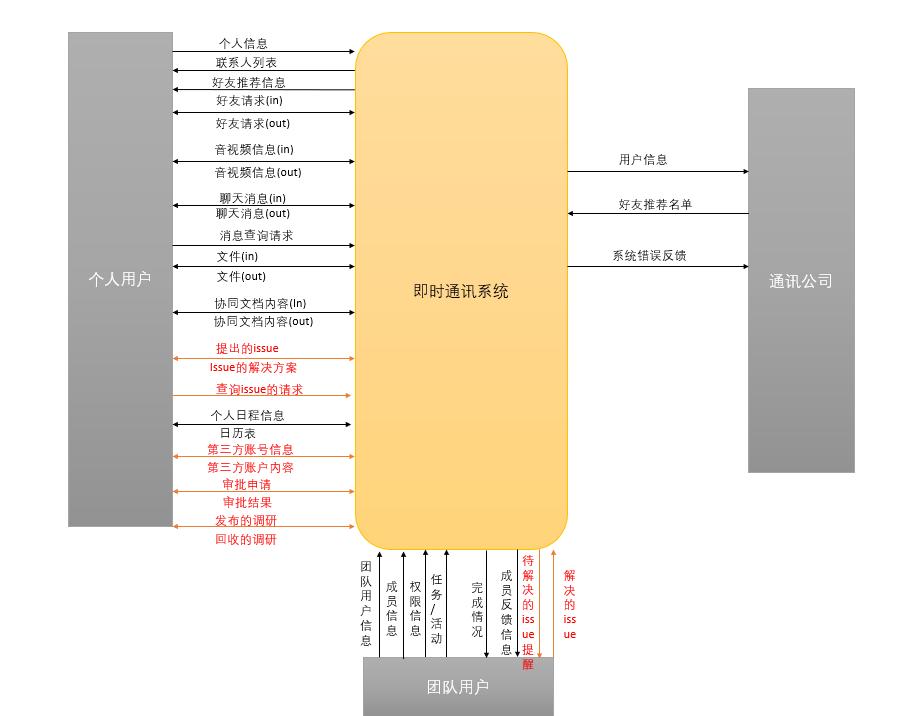
\includegraphics[scale = 0.75]{top_level_new.png}\label{tab:classification}
            \caption{\color{red} 顶层数据流图}\label{fig:noted-figure}
            \note{\color{red} 本图片说明了数据在实体与系统之间的流动}
        \end{figure}
    \end{landscape}
        \newpage
    \begin{landscape}
        \subsection{\color{red} 0层数据流图}
        %======================================================================================
        % 在这里画出0层数据流图
        注:图中修改的地方用红色标出了
        \begin{figure}[ht]
            \centering
            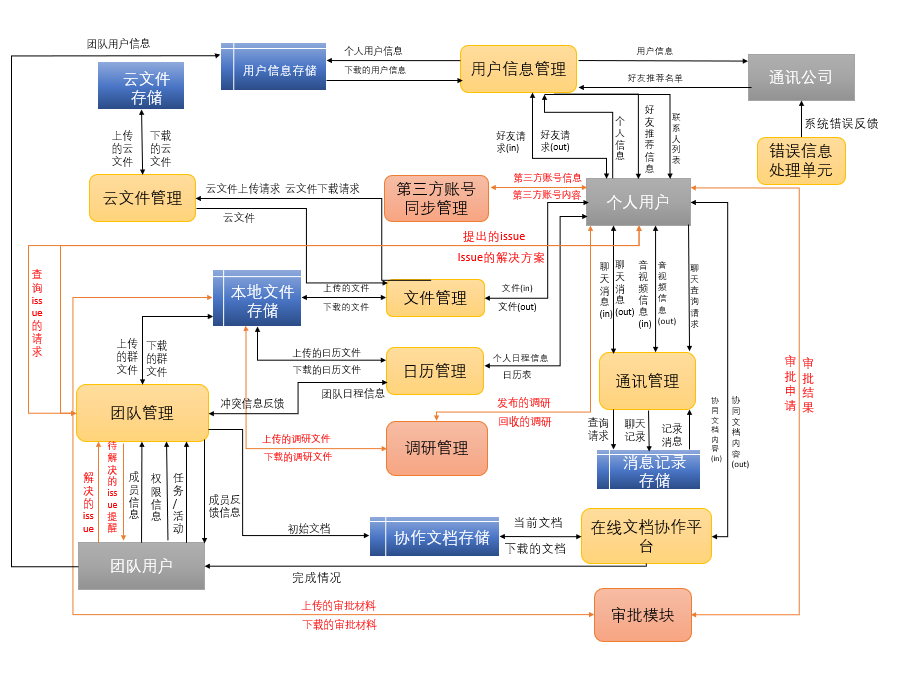
\includegraphics[scale = 0.75]{0_level_new.png}\label{tab:classification}
            \caption{\color{red} 0层数据流图}\label{fig:noted-figure}
            \note{\color{red} 本图片细化说明了数据在实体,加工,存储之间的流动}
        \end{figure}
        %======================================================================================
    \end{landscape}
        \newpage
%======================================================================================
    \section{\color{red} 数据字典}

        \subsection{\color{red} 数据流说明}
            
            %======================================================================================
            % 与数据流图中的名称一致,采用数据描述符号说明数据流的内容
            %===========================================================
            % 个人用户
            %======================================================================================
            {\color{red}
            \subsubsection{\color{red} 审批申请}
            \begin{itemize}
                \item 来源:个人用户
                \item 去向:审批模块
                \item 内容:审批申请 = 申请编号 + 申请标题 + 申请材料
                \item 数据类型:\\
                    申请编号 = \{0...9\}\\
                    申请标题 = \{char\}\\
                    申请材料 = 二进制文件包\\
            \end{itemize}

            \subsubsection{\color{red} 审批过程查询}
            \begin{itemize}
                \item 来源:个人用户
                \item 去向:审批模块
                \item 内容:审批过程查询 = [审批编号,审批标题]
                \item 数据类型:\\
                    审批编号 = \{0...9\}\\
                    审批标题 = \{char\}\\
            \end{itemize}
            
            \subsubsection{\color{red} 审批结果}
            \begin{itemize}
                \item 来源:审批模块
                \item 去向:个人用户
                \item 内容:审批结果 = 审批编号 + 审批标题 + 审批结果
                \item 数据类型:\\
                    审批编号 = \{0...9\}\\
                    审批标题 = \{char\}\\
                    审批结果 = \{char\}\\
            \end{itemize}
            \subsubsection{\color{red} 第三方账号信息}
            \begin{itemize}
                \item 来源:个人用户
                \item 去向:第三方账号同步管理
                \item 内容:第三方账号信息 = 用户账号 + 第三方平台账号 + 第三方平台登陆密码
                \item 数据类型:\\
                    用户账号 = \{0...9\}\\
                    第三方平台账号 = \{0...9\}\\
                    第三方平台登陆密码 = \{char\}\\
            \end{itemize}
            \subsubsection{\color{red} 第三方账户内容}
            \begin{itemize}
                \item 来源:第三方账号同步管理
                \item 去向:个人用户
                \item 内容:第三方账户内容 = 用户账号 + 第三方平台账号 + 第三方平台消息
                \item 数据类型:\\
                    用户账号 = \{0...9\}\\
                    第三方平台账号 = \{0...9\}\\
                    第三方平台消息 = 二进制数据包\\
            \end{itemize}
            \subsubsection{\color{red} 提出的issue}
            \begin{itemize}
                \item 来源:个人用户
                \item 去向:团队管理
                \item 内容:提出的issue = 提出者账号 + 提出时间 + issue内容
                \item 数据类型:\\
                    提出者账号 = \{0...9\}\\
                    提出时间 = time\\
                    issue内容 = \{char\}\\
            \end{itemize}
            \subsubsection{\color{red} 查询issue的请求}
            \begin{itemize}
                \item 来源:个人用户
                \item 去向:团队管理
                \item 内容:提出的issue = 查询者账号 + [issue编号 | issue内容 ]
                \item 数据类型:\\
                    查询者账号 = \{0...9\}\\
                    issue编号 = \{0...9\}\\
                    issue内容 = \{char\}\\
            \end{itemize}
            \subsubsection{\color{red} issue的解决方案}
            \begin{itemize}
                \item 来源:团队管理
                \item 去向:个人用户
                \item 内容:issue的解决方案 = issue编号 + issue内容 + 解决方案内容
                \item 数据类型:\\
                    issue编号 = \{0...9\}\\
                    issue内容 = \{char\}\\
                    解决方案内容 = \{char\}\\
            \end{itemize}
            \subsubsection{\color{red} 发布的调研}
            \begin{itemize}
                \item 来源:个人用户
                \item 去向:调研管理
                \item 内容:发布的调研 = 调研标题 + 调研方式 + {受访人表} + 调查问卷 + 时间限制
                \item 数据类型:\\
                    调研标题 = \{char\}\\
                    调研方式 = ["所有人可见" | "部分人可见"] \\
                    受访人表 = \{账号\}\\
                    账号 = \{0...9\}\\
                    调查问卷 = 二进制文件包 \\
                    时间限制 = time \\
            \end{itemize}
            \subsubsection{\color{red} 回收的调研}
            \begin{itemize}
                \item 来源:调研管理
                \item 去向:个人用户
                \item 内容:回收的调研 = 调研标题 + 调研结果
                \item 数据类型:\\
                    调研标题 = \{char\}\\
                    调研结果 = 二进制文件包\\
            \end{itemize}
            
            \subsubsection{\color{red} 上传的调研文件}
            \begin{itemize}
            \item 来源:调研管理
            \item 去向:本地文件存储
            \item 内容:调研文件 = 用户账号 + 调研编号 + 文件
            \item 数据类型:\\
            用户账号 = \{0...9\}\\
            调研编号 = \{0...9\}\\
            文件 = 二进制数据包\\
            \end{itemize}

            \subsubsection{\color{red} 下载的调研文件}
            \begin{itemize}
            \item 来源:本地文件存储
            \item 去向:调研管理
            \item 内容:调研文件 = 用户账号 + 调研编号 + 文件
            \item 数据类型:\\
            用户账号 = \{0...9\}\\
            调研编号 = \{0...9\}\\
            文件 = 二进制数据包\\
            \end{itemize}

            \subsubsection{\color{red} 上传的审批材料}
            \begin{itemize}
            \item 来源:审批模块
            \item 去向:本地文件存储
            \item 内容:审批材料 = 申请者账号 + 审批者账号 + 审批编号 + \{文件\}
            \item 数据类型:\\
            申请者账号 = \{0...9\}\\
            审批者账号 = \{0...9\}\\
            审批编号 = \{0...9\}\\
            文件 = 二进制数据包\\
            \end{itemize}

            \subsubsection{\color{red} 下载的审批材料}
            \begin{itemize}
            \item 来源:本地文件存储
            \item 去向:审批模块
            \item 内容:审批材料 = 申请者账号 + 审批者账号 + 审批编号 + \{文件\}
            \item 数据类型:\\
            申请者账号 = \{0...9\}\\
            审批者账号 = \{0...9\}\\
            审批编号 = \{0...9\}\\
            文件 = 二进制数据包\\
            \end{itemize}

            \subsubsection{\color{red} 待解决的issue提醒}
            \begin{itemize}
            \item 来源:团队管理
            \item 去向:团队用户
            \item 内容:待解决的issue提醒 = \{issue编号 + issue内容\} 
            \item 数据类型:\\
            issue编号 = \{0...9\}\\
            issue内容 = \{char\}\\
            \end{itemize}
            
            \subsubsection{\color{red} 解决的issue}
            \begin{itemize}
            \item 来源:团队用户
            \item 去向:团队管理
            \item 内容:解决的issue = issue编号 + issue的解决方案
            \item 数据类型:\\
            issue编号 = \{0...9\}\\
            issue的解决方案 = \{char\}\\
            \end{itemize}
            }

            % ===================== old =================%

            \subsubsection{音视频信息(out)}
            \begin{itemize}
                \item 来源:个人用户
                \item 去向:通讯管理
                \item 内容:音视频信息(out) = [音频聊天请求(out) | 视频聊天请求(out) | 音频聊天数据流 | 视频聊天数据流]
                \item 数据类型:\\
                    二进制数据包\\
            \end{itemize}
            \subsubsection{音视频信息(in)}
            \begin{itemize}
                    \item 来源:通讯管理
                    \item 去向:个人用户
                    \item 内容:音视频信息(in) = [音频聊天请求(in) | 视频聊天请求(in) | 音频聊天数据流 | 视频聊天数据流]
                    \item 数据类型:\\
                    二进制数据包\\
            \end{itemize}
            \subsubsection{好友请求(out)}
            \begin{itemize}
                \item 来源:个人用户
                \item 去向:用户信息管理
                \item 内容:好友请求(out) = [申请添加联系人信息 | 申请加入群组信息 | 同意添加申请人信息 | 同意加入群组信息]
                \item 数据类型:\\
                \{char\}\\
            \end{itemize}
                \subsubsection{好友请求(in)}
                \begin{itemize}
                    \item 来源:用户信息管理
                    \item 去向:个人用户
                    \item 内容:好友请求(in) = [被申请加为联系人信息 | 被邀请加入群组信息]
                    \item 数据类型:\\{char}
            \end{itemize}
            \subsubsection{聊天消息(out)}
            \begin{itemize}
                \item 来源:个人用户
                \item 去向:通讯管理
                \item 内容:聊天信息(out) = 己方账号 + \{char,image\} + 发出时间
                \item 数据类型:\\己方账号 = \{0...9\}\\
                         发出时间 = time
            \end{itemize}
            \subsubsection{聊天消息(in)}
            \begin{itemize}
                \item 来源:通讯管理
                \item 去向:个人用户
                \item 内容:聊天信息(in) = 对方账号 + \{char,image\} + 接收时间
                \item 数据类型:\\
                己方账号 = \{0...9\}\\
                接收时间 = time\\
            \end{itemize}
            \subsubsection{消息查询请求}
            \begin{itemize}
                \item 来源:个人用户
                \item 去向:通讯用户
                \item 内容:消息查询请求 = 己方账号 + 被查询方账号 + 查询信息
                \item 数据类型:\\
                      账号 = \{0...9\}\\
                      查询信息 = [time | \{char\}]\\
            \end{itemize}
            \subsubsection{文件(out)}
            \begin{itemize}
                \item 来源:文件管理
                \item 去向:个人用户
                \item 内容:文件(out) = 己方账号 + 文件 + 发出时间
                \item 数据类型:\\
                账号 = \{0...9\}\\
                文件 = 二进制文件包\\
                发出时间 = time\\
            \end{itemize}
            \subsubsection{文件(in)}
            \begin{itemize}
                \item 来源:个人用户
                \item 去向:文件管理
                \item 内容:文件(out) = 对方账号 + 文件 + 接收时间
                \item 数据类型:\\
                账号 = \{0...9\}\\
                文件 = 二进制文件包\\
                接收时间 = time\\
            \end{itemize}
            \subsubsection{协同文档内容(out)}
            \begin{itemize}
                \item 来源:个人用户
                \item 去向:在线文档协作平台
                \item 内容:协同文档内容(out) = 己方账号 + 修改内容 + 修改时间 + 修改信息
                \item 数据类型:\\
                账号 = \{0...9\}\\
                修改内容 = \{char, image\}\\
                修改时间 = time\\
                修改信息 = \{char\}\\
            \end{itemize}
            \subsubsection{协同文档内容(in)}
            \begin{itemize}
                \item 来源:在线文档协作平台
                \item 去向:个人用户
                \item 内容:协同文档内容(out) = 当前文档
                \item 数据类型:\\
                当前文档 = \{char,image\}\\
            \end{itemize}
            \subsubsection{个人信息}
            \begin{itemize}
                \item 来源:个人用户
                \item 去向:用户信息管理
                \item 内容:个人信息 = 己方账号 + 己方信息
                \item 数据类型:\\
                账号 = \{0...9\}\\
                己方信息 = [邮箱 | 手机号 | 头像 | 住址 | 证件号]\\
            \end{itemize}
            \subsubsection{个人日程信息}
            \begin{itemize}
                \item 来源:个人用户
                \item 去向:日历管理
                \item 内容:个人日程信息 = 己方账号 + 日程信息变动
                \item 数据类型:\\
                账号 = \{0...9\}\\
                日程信息变动 = \{时间 + 事件\}\\
            \end{itemize}
            \subsubsection{日历表}
            \begin{itemize}
                \item 来源:日历管理
                \item 去向:个人用户
                \item 内容:日历表 = \{时间 + 事件\}
                \item 数据类型:\\
                时间 = time\\
                事件 = \{char\}\\
            \end{itemize}
            \subsubsection{好友推荐信息}
            \begin{itemize}
                \item 来源:用户信息管理
                \item 去向:个人用户
                \item 内容:好友推荐信息 = 对方账号 + 对方档案
                \item 数据类型:\\
                账号 = \{0...9\}\\
                对方档案 = 档案结构体\\
            \end{itemize}
            \subsubsection{联系人列表}
            \begin{itemize}
                \item 来源:用户信息管理
                \item 去向:个人用户
                \item 内容:联系人列表 = \{联系人档案\}
                \item 数据类型:\\
                联系人档案 = 档案结构体\\
            \end{itemize}
            %=======================================================
            % 团队用户
            %===========================================================
            \subsubsection{任务/活动}
            \begin{itemize}
                \item 来源:团队用户
                \item 去向:团队管理
                \item 内容:任务/活动 = \{发布者信息 + [任务 | 活动] + 发布时间\}
                \item 数据类型:\\
                发布者信息 = 档案结构体\\
                任务 = \{char, image\}\\
                活动 = \{char, image\}\\
                发布时间 = time\\
            \end{itemize}
            \subsubsection{成员信息}
            \begin{itemize}
                \item 来源:团队用户
                \item 去向:团队管理
                \item 内容:成员信息 = 成员名单变动\\
                    成员名单变动 = [添加的成员名单 | 删除的成员名单]\\
                    成员名单 = \{账号\}\\
                \item 数据类型:\\
                    账号 = \{0...9\}\\
            \end{itemize}
            \subsubsection{权限信息}
            \begin{itemize}
                \item 来源:团队用户
                \item 去向:团队管理
                \item 内容:权限信息 = \{成员账号 + 成员权限\}
                \item 数据类型:\\
                账号 = \{0...9\} \\
                成员权限 = \{char\} \\
            \end{itemize}
            \subsubsection{完成情况}
            \begin{itemize}
                \item 来源:在线文档协作平台
                \item 去向:团队用户
                \item 内容:完成情况 = 当前时间 + \{成员账号 + 成员已完成比例\}
                \item 数据类型:\\
                时间 = time \\
                账号 = \{0...9\} \\
                完成比例 = float \\
            \end{itemize}
            \subsubsection{成员反馈信息}
            \begin{itemize}
                \item 来源:团队管理
                \item 去向:团队用户
                \item 内容:成员反馈信息 = \{反馈者账号 + 反馈内容 + 反馈时间\}
                \item 数据类型:\\
                账号 = \{0...9\} \\
                反馈内容 = \{char, image\} \\
                反馈时间 = time\\
            \end{itemize}
            \subsubsection{团队用户信息}
            \begin{itemize}
                \item 来源:团队用户
                \item 去向:用户信息管理
                \item 内容:团队用户信息 = \{团队成员 + 权限信息 + 任务活动历史\} \\
                     权限信息 = \{成员账号 + 成员权限\}\\
                     任务活动历史 = \{任务活动名称 + 任务活动内容 + 发布时间 + 完成时间\}\\
                \item 数据类型:\\
                账号 = \{0...9\}\\
                成员权限 = \{char\}\\
                任务活动名称 = \{char\}\\
                任务活动内容 = \{char\}\\
                发布时间 = time\\
                完成时间 = time\\
            \end{itemize}
            %=======================================================
            % 通讯公司
            %===========================================================
            \subsubsection{用户信息}
            \begin{itemize}
                \item 来源:用户信息管理
                \item 去向:通讯公司
                \item 内容:用户信息 = \{用户档案\}
                \item 数据类型:用户档案 = 档案结构体
            \end{itemize}
            \subsubsection{好友推荐名单}
            \begin{itemize}
                \item 来源:通讯公司
                \item 去向:用户信息管理
                \item 内容:好友推荐名单 = \{推荐好友档案\}
                \item 数据类型:推荐好友档案 = 档案结构体
            \end{itemize}
            \subsubsection{系统错误反馈}
            \begin{itemize}
                \item 来源:错误信息处理单元
                \item 去向:通讯公司
                \item 内容:错误信息 = \{错误位置 + 错误时间 + 错误内容\}
                \item 数据类型:\\
                错误位置 = \{char\}\\
                错误时间 = time\\
                错误内容 = \{char\}\\
            \end{itemize}
            %=======================================================
            % 云文件管理中间
            %===========================================================
            \subsubsection{上传的云文件}
            \begin{itemize}
            \item 来源:云文件管理
            \item 去向:云文件存储
            \item 内容:上传的云文件 = \{用户账号 + 文件\}
            \item 数据类型:\\
            账号 = \{0...9\}\\
            文件 = 二进制数据包\\
            \end{itemize}

            \subsubsection{下载的云文件}
            \begin{itemize}
            \item 来源:云文件存储
            \item 去向:云文件管理
            \item 内容:下载的云文件 = \{用户账号 + 文件\}
            \item 数据类型:\\
            账号 = \{0...9\}\\
            文件 = 二进制数据包\\
            \end{itemize}

            \subsubsection{云文件上传请求}
            \begin{itemize}
            \item 来源:文件管理
            \item 去向:云文件管理
            \item 内容:云文件上传请求 = \{用户账号 + 请求信息 + 文件\}
            \item 数据类型:\\
            账号 = \{0...9\}\\
            请求信息 = \{char\}\\
            文件 = 二进制数据包\\
            \end{itemize}

            \subsubsection{云文件下载请求}
            \begin{itemize}
            \item 来源:文件管理
            \item 去向:云文件管理
            \item 内容:云文件下载请求 = \{用户账号 + 请求信息 + 文件\}
            \item 数据类型:\\
            账号 = \{0...9\}\\
            请求信息 = \{char\}\\
            文件 = 二进制数据包\\
            \end{itemize}

            \subsubsection{云文件}
            \begin{itemize}
            \item 来源:云文件管理
            \item 去向:文件管理
            \item 内容:云文件 = \{用户账号 + 文件\}
            \item 数据类型:\\
            账号 = \{0...9\}\\
            文件 = 二进制数据包\\
            \end{itemize}
            %=======================================================
            % 本地文件存储中间
            %===========================================================
            \subsubsection{上传的文件}
            \begin{itemize}
            \item 来源:文件管理
            \item 去向:本地文件存储
            \item 内容:文件 = \{用户账号 + 文件\}
            \item 数据类型:\\
            账号 = \{0...9\}\\
            文件 = 二进制数据包\\
            \end{itemize}

            \subsubsection{上传的群文件}
            \begin{itemize}
            \item 来源:团队管理
            \item 去向:本地文件存储
            \item 内容:文件 = \{群账号 + 文件 + 发送者账号\}
            \item 数据类型:\\
            账号 = \{0...9\}\\
            文件 = 二进制数据包\\
            \end{itemize}

            \subsubsection{上传的日历文件}
            \begin{itemize}
            \item 来源:日历管理
            \item 去向:本地文件存储
            \item 内容:日历文件 = 用户账号 + \{时间 + 事件\}
            \item 数据类型:\\
            账号 = \{0...9\}\\
            时间 = time\\
            事件 = \{char\}\\
            \end{itemize}

            \subsubsection{下载的文件}
            \begin{itemize}
            \item 来源:本地文件存储
            \item 去向:文件管理
            \item 内容:文件 = \{用户账号 + 文件\}
            \item 数据类型:\\
            账号 = \{0...9\}\\
            文件 = 二进制数据包\\
            \end{itemize}

            \subsubsection{下载的群文件}
            \begin{itemize}
            \item 来源:本地文件存储
            \item 去向:团队管理
            \item 内容:文件 = \{群账号 + 文件 + 发送者账号\}
            \item 数据类型:\\
            账号 = \{0...9\}\\
            文件 = 二进制数据包\\
            \end{itemize}

            \subsubsection{下载的日历文件}
            \begin{itemize}
            \item 来源:本地文件存储
            \item 去向:日历管理
            \item 内容:日历文件 = 用户账号 + \{时间 + 事件\}
            \item 数据类型:\\
            账号 = \{0...9\}\\
            时间 = time\\
            事件 = \{char\}\\
            \end{itemize}
            %=======================================================
            % 日历文件存储中间
            %===========================================================
            \subsubsection{团队日程信息}
            \begin{itemize}
            \item 来源:团队管理
            \item 去向:日历管理
            \item 内容:团队日程信息 = 团队账号 + \{时间 + 事件\}
            \item 数据类型:\\
            账号 = \{0...9\}\\
            时间 = time\\
            事件 = \{char\}\\
            \end{itemize}

            \subsubsection{冲突信息反馈}
            \begin{itemize}
            \item 来源:日历管理
            \item 去向:团队管理
            \item 内容:冲突信息反馈 = {冲突者账号 + 冲突时间 + 冲突事件}
            \item 数据类型:\\
            账号 = \{0...9\}\\
            时间 = time\\
            事件 = \{char\}\\
            \end{itemize}
            %=======================================================
            % 消息记录存储中间
            %===========================================================
            \subsubsection{聊天记录}
            \begin{itemize}
            \item 来源:通讯管理
            \item 去向:消息记录存储
            \item 内容:聊天记录 = 发送者账号 + 接收者账号 + 聊天内容 + 聊天时间
            \item 数据类型:\\
            账号 = \{0...9\}\\
            时间 = time\\
            聊天内容 = \{[char, image]\}\\
            \end{itemize}

            \subsubsection{查询请求}
            \begin{itemize}
            \item 来源:通讯管理
            \item 去向:消息记录存储
            \item 内容:查询请求 = 查询方账号 + 被查询方账号 + (关键字)
            \item 数据类型:\\
            账号 = \{0...9\}\\
            关键字 = \{char\}\\
            \end{itemize}

            \subsubsection{记录消息}
            \begin{itemize}
            \item 来源:消息记录存储
            \item 去向:通讯管理
            \item 内容:记录消息 = 发送者账号 + 接收者账号 + 聊天内容 + 聊天时间
            \item 数据类型:\\
            账号 = \{0...9\}\\
            聊天时间 = time\\
            聊天内容 = \{[char, image]\}\\
            \end{itemize}
            %=======================================================
            % 协作文档存储中间
            %===========================================================
            \subsubsection{初始文档}
            \begin{itemize}
            \item 来源:群组管理
            \item 去向:协作文档存储
            \item 内容:初始文档 = 文档 + 发布时间
            \item 数据类型:\\
            文档 = \{char, image\}\\
            时间 = time\\
            
            \end{itemize}

            \subsubsection{总文档}
            \begin{itemize}
            \item 来源:在线文档协作平台
            \item 去向:协作文档存储
            \item 内容:总文档 = 文档 + 修改时间
            \item 数据类型:\\
            文档 = \{char, image\}\\
            时间 = time\\
            
            \end{itemize}

            \subsubsection{文档任务}
            \begin{itemize}
            \item 来源:协作文档存储
            \item 去向:在线文档协作平台
            \item 内容:文档任务 = \{任务责任人账号 + 任务内容\}
            \item 数据类型:\\
            任务责任人账号 = \{0...9\}\\
            任务内容 = \{char\}\\
              
            \end{itemize}


        \subsection{\color{red} 数据存储说明}
        {\color{red}
            \subsubsection{\color{red} issue记录存储}
            \begin{itemize}
            \item 说明:存储每个团队中的issue与其解决方案
            \item 编号:D0
            \item 输入数据流:上传的issue
            \item 输出数据流:下载的issue
            \item 排列方式:按照已解决和未解决分类存储。每一类中按照时间顺序存储。\\
                           存储单元:issue编号+issue状态+issue内容+issue的解决方案\\
            \end{itemize}
        }
            \subsubsection{本地文件存储}
            \begin{itemize}
                \item 说明:存储用户之间传送的文件,位于本地的存储空间中
                \item 编号:D1
                \item 输入数据流:[上传的群文件,上传的日历文件, 上传的文件]
                \item 输出数据流:[下载的群文件,下载的日历文件, 下载的文件]
                \item 排列方式:群文件按照群分组,按照日期排列,索引为群账号+文件名\\
                               个人文件按照发送用户分组,按照日期排列,索引为用户账号+文件名\\
                               日历文件按照用户分组,索引为用户账号+日历标记\\
                               存储单元:发送者+(接收者)+文件名+文件\\
            \end{itemize}
            \subsubsection{云文件存储}
            \begin{itemize}
                \item 说明:存储用户之间传送的文件,位于云端的存储空间中
                \item 编号:D2
                \item 输入数据流:[云文件上传请求,云文件下载请求,下载的云文件]
                \item 输出数据流:[云文件,上传的云文件]
                \item 排列方式:群文件按照群分组,按照日期排列,索引为群账号+文件名\\
                               个人文件按照发送用户分组,按照日期排列,索引为用户账号+文件名\\
                               日历文件按照用户分组,索引为用户账号+日历标记\\
                               存储单元:发送者+(接收者)+文件名+文件\\
            \end{itemize}
            \subsubsection{消息记录存储}
            \begin{itemize}
                \item 说明:存储用户的消息记录
                \item 编号:D3
                \item 输入数据流:[聊天记录,查询请求]
                \item 输出数据流:记录消息
                \item 排列方式:按照发送者分组,按照日期排列,索引为发送者+发送时间+接收者\\
                         存储单元:发送者+发送时间+接收者+聊天记录\\
            \end{itemize}
            \subsubsection{用户信息存储}
            \begin{itemize}
                \item 说明:存储用户的档案信息,例如账号,姓名,联系方式等
                \item 编号:D4
                \item 输入数据流:[个人用户信息,团队用户信息]
                \item 输出数据流:[下载的用户信息]
                \item 排列方式:个人用户信息按照用户账号排列,索引为用户账号\\
                               团队用户信息按照团队账号排列,索引为团队账号\\
                               存储单元:账号+[个人标识,团队标识]+联系人列表+头像+邮箱+手机号+个人简介\\
            \end{itemize}
            \subsubsection{协作文档存储}
            \begin{itemize}
                \item 说明:存储过期时间之前的协作文档
                \item 编号:D5
                \item 输入数据流:[初始文档, 当前文档]
                \item 输出数据流:下载的文档
                \item 排列方式:按照发布者账号分组,组内按照最近更改时间排序,索引为发布者账号+文档名\\
                         存储单元:发布者账号+文档名+发布时间+最近更改时间+成员信息+文档内容\\
            \end{itemize}
            %======================================================================================
            % 与数据流图中的名称一致,采用数据描述符号说明数据流的内容,另外还需描述数据排列方式
            %======================================================================================
        \subsection{\color{red} 加工说明}
        {\color{red}
        \subsubsection{\color{red} 第三方账号同步管理}
        \begin{itemize}
            \item 说明:使用第三方平台接口,在即时通讯软件中同步第三方账号,同步获取第三方平台的内容
            \item 输入数据流:第三方账号信息
            \item 输出数据流:第三方账号内容
            \item 激发条件:用户在软件中登陆第三方平台(发送账号信息和密码)
            \item 处理过程:
%=====================================================================================================
\begin{lstlisting}[language=C, caption=错误信息处理单元, label={code:first-code}]
IF(用户登陆):
调用第三方平台API
登陆第三方账号
爬取第三方平台内容
返回内容
\end{lstlisting}
%=====================================================================================================
        \end{itemize}

\subsubsection{\color{red} 调研管理}
        \begin{itemize}
            \item 说明:管理用户发布的调研表,投票,问卷等。
            \item 输入数据流:[发布的调研,下载的调研文件]
            \item 输出数据流:[回收的调研,上传的调研文件]
            \item 激发条件:有新的调研发布或调研的结束条件被满足(例如:期限到达)
            \item 处理过程:
%=====================================================================================================
\begin{lstlisting}[language=C, caption=错误信息处理单元, label={code:first-code}]
IF(新的调研):
    将新的调研加入缓存;
    向本地文件存储上传调研文件;
    向目标用户群体发送调研信息;

ELSE IF(调研结束):
    下载调研文件;
    整合调研信息;
    返回回收的调研

\end{lstlisting}
%=====================================================================================================
        \end{itemize}
\subsubsection{\color{red} 审批模块}
        \begin{itemize}
            \item 说明:管理用户的审批申请,审批流程的追踪,审批结果记录。例如项目审批,报销审批等。
            \item 输入数据流: [审批申请,审批过程查询,下载的审批材料]
            \item 输出数据流:[审批结果,上传的审批材料]
            \item 激发条件:出现审批申请或审批过程查询或收到审批结果
            \item 处理过程:
%=====================================================================================================
\begin{lstlisting}[language=C, caption=错误信息处理单元, label={code:first-code}]
IF(审批申请):
    将审批加入缓存表;
    向本地文件存储上传审批材料;
    将审批材料和审批记录发送给审批者;

ELSE IF(审批过程查询):
    从缓存表中查找对应的审批项;
    IF(找到) 返回当前的审批结果表
    ELSE 返回“该审批不存在”

ELSE IF(收到审批结果):
    从缓存表中查找对应的审批项;
    向该项中加入该审批结果;
    IF(审批结束) 向用户返回审批结果表
\end{lstlisting}
%=====================================================================================================
        \end{itemize}
        }
            \subsubsection{文件管理}
            \begin{itemize}
                \item 说明:响应用户的传输文件需求,并将文件组织好放置于存储中
                \item 输入数据流:[文件(in), 下载的文件,云文件]
                \item 输出数据流:[文件(out), 上传的文件,云文件上传请求,云文件下载请求]
                \item 激发条件:有文件传输请求;有用户的下载请求
                \item 处理过程:
%=====================================================================================================
\begin{lstlisting}[language=C, caption=文件管理, label={code:first-code}]
IF(有文件传输请求):
    检验发送方合法性;
    检验接受方合法性;
    接受文件;
    将文件包装为 发送方 文件 接受方 发送时间的格式;
IF(本地存储已满) 
    将文件上传到云端存储中
ELSE 
    将文件上传到本地存储中;
    发送文件;
                
IF(有用户下载请求):
    检验用户合法性;
    计算文件存储地址;
    IF(文件不存在) 
        向用户返回错误信息;
    ELSE IF(地址在本地)
        访问本地文件存储
        发送文件
    ELSE 
        向云文件管理发送云文件下载请求;
        接受云文件;
        发送文件
\end{lstlisting}
%=====================================================================================================
            \end{itemize}    
            \subsubsection{云文件管理}
            \begin{itemize}
                \item 说明:管理云端文件的上传和下载
                \item 输入数据流:[云文件上传请求,云文件下载请求,下载的云文件]
                \item 输出数据流:云文件,上传的云文件
                \item 激发条件:收到云文件上传请求或云文件下载请求
                \item 处理过程: 
%=====================================================================================================
\begin{lstlisting}[language=C, caption=云文件管理, label={code:first-code}]
IF(云文件上传请求):
    分配地址;
    上传云文件
IF(云文件下载请求):
    计算物理地址;
    取文件;
    返回云文件
\end{lstlisting}
%=====================================================================================================
            \end{itemize}
            \subsubsection{日历管理}
            \begin{itemize}
                \item 说明:个人用户制订个人日历,团队用户可以在该成员的日历上添加任务与活动信息
                \item 输入数据流:[个人日程信息,团队日程信息,下载的日历文件]
                \item 输出数据流:[日历表,上传的日程信息,冲突信息反馈]
                \item 激发条件:有个人日程信息或团队日程信息输入
                \item 处理过程:
%=====================================================================================================
\begin{lstlisting}[language=C, caption=日历管理, label={code:first-code}]
IF(输入个人日程信息):
    检查与原日历表是否冲突;
    IF(冲突) 
        向个人返回冲突信息;
    ELSE:
        向日日历中加入该日程;
        上传新的日历文件;
        返回新的日历文件
ELSE(输入团队日程信息)
    FOR(成员 in 团队)
        下载该成员的日历
        检查与该成员原日历表是否冲突;
            IF(冲突) 
                向团队返回冲突信息;
                结束任务;
                    
    FOR(成员 in 团队)
        向该成员日历中加入该日程;
        上传新的日历文件;
        向该成员发送新的日历文件
\end{lstlisting}
%=====================================================================================================
            \end{itemize}
            \subsubsection{团队管理}
            \begin{itemize}
                \item 说明:管理团队的成员,发布与管理团队的任务活动
                \item 输入数据流:[成员信息,权限信息,任务活动,冲突信息反馈,下载的群文件]
                \item 输出数据流:[团队用户信息,成员反馈信息,初始文档,团队日程信息,上传的群文件,]
                \item 激发条件:有成员信息,权限信息,任务活动传入
                \item 处理过程:
%=====================================================================================================
\begin{lstlisting}[language=C, caption=团队管理, label={code:first-code}]
IF(成员信息):
    IF(添加成员):
        向团队用户信息中添加成员
        输出团队用户信息
    ELSE IF(删除成员):
        从团队用户信息中删除成员
        输出团队用户信息
    ELSE IF(修改成员):
        在团队用户信息中修改成员
        输出团队用户信息
    ELSE IF(查询成员):
        从存储中下载成员信息
        输出查询成员信息
IF(权限信息):
    修改对应成员的权限信息
    更新团队信息
IF(任务活动):
    发出团队日程信息;
IF(是文档任务)
    发布初始文档
    更新团队信息
IF(冲突信息反馈):
    重新指定对应任务
    发布新的团队日程信息
    更新团队信息
IF(群文件):
    上传群文件
\end{lstlisting}
%=====================================================================================================                      
            \end{itemize}
            \subsubsection{通讯管理}
            \begin{itemize}
                \item 说明:基本功能。用户之间发送信息进行通讯
                \item 输入数据流:[聊天消息(out),音视频信息(out),消息查询请求,记录消息]
                \item 输出数据流:[聊天消息(in),音视频信息(in),聊天记录,查询请求]
                \item 激发条件:有消息输入;有用户上线
                \item 处理过程: 
%=====================================================================================================
\begin{lstlisting}[language=C, caption=通讯管理, label={code:first-code}]
IF(传入聊天消息):
    IF(对方用户在线):
        立刻转发给对方用户
    ELSE:
        缓存信息 对方用户上线时转发给对方
    将聊天记录上传到存储中
ELSE IF(传入音视频信息):
    立即发送给对方
    IF(未收到对方反馈):
        中断音视频连接
ELSE IF(消息查询请求):
    从存储中下载记录消息
    将记录消息返回
ELSE IF(用户上线)
    查询缓存,发送离线信息
\end{lstlisting}
%=====================================================================================================
            \end{itemize}
            \subsubsection{用户信息管理}
            \begin{itemize}
                \item 说明:实现用户信息的绑定,好友推荐的信息处理,好友请求,联系人列表管理等和用户信息有关的功能
                \item 输入数据流:[好友请求(out),好友推荐名单,个人信息,下载的用户信息]
                \item 输出数据流:[好友请求(in),好友推荐信息,个人用户信息,用户信息]
                \item 激发条件:有信息输入;有用户上线
                \item 处理过程: 
%=====================================================================================================
\begin{lstlisting}[language=C, caption=用户信息管理, label={code:first-code}]
IF(好友请求)
    IF(对方用户在线):
        立刻转发给对方用户
    ELSE:
        缓存信息 对方用户上线时转发给对方
ELSE IF(个人信息)
    将个人信息上传到用户信息存储中,绑定到对应的用户
ELSE IF(好友推荐名单)
    下载名单中用户的用户信息
    将推荐用户及其部分信息转发给对应用户
ELSE IF(有用户上线)
    将该用户的联系人列表发送给用户
    将缓存的离线信息发送给对应用户
\end{lstlisting}
%=====================================================================================================
             \end{itemize}
            \subsubsection{在线文档协作平台}
            \begin{itemize}
                \item 说明:可以多人同时编辑文档
                \item 输入数据流:[协作文档内容(out),下载的文档]
                \item 输出数据流:[协作文档内容(in),当前文档,完成情况]
                \item 激发条件:有文档/文档的增删改查传入
                \item 处理过程: 
%=====================================================================================================
\begin{lstlisting}[language=C, caption=在线文档协作平台, label={code:first-code}]
IF(布置新的文档)
    更新完成情况
ELSE IF(文档增加内容)
    增加文档
    返回最新的协作文档内容
    上传当前文档
    更新完成情况
ELSE IF(文档删除内容)
    删除文档
    返回最新的协作文档内容
    上传当前文档
    更新完成情况
ELSE IF(文档修改内容)
    修改文档
    返回最新的协作文档内容
    上传当前文档
    更新完成情况
\end{lstlisting}
%=====================================================================================================
            \end{itemize}
            \subsubsection{错误信息处理单元}
            \begin{itemize}
                \item 说明:系统中的每个元件返回的错误信息,例如存储空间不足,系统版本不兼容等
                \item 输入数据流:所有元件的错误信息(因为每个元件都有,为了图的简洁,在图中未标出)
                \item 输出数据流:系统错误反馈
                \item 激发条件:有错误信息到来
                \item 处理过程:
%=====================================================================================================
\begin{lstlisting}[language=C, caption=错误信息处理单元, label={code:first-code}]
IF(错误信息):
    记录错误来源与错误类型
    向公司反馈错误
    采用应急预案
\end{lstlisting}
%=====================================================================================================
            \end{itemize}




            %======================================================================================
            % 采用自然语言,判断表/判断树,伪码的形式描述对数据流进行处理的过程
            %======================================================================================
%======================================================================================